
\clearpage{}
% -----------------------------------------------------------------------------
\section{Privacy}
\label{s:Privacy}

\begin{figure}
\begin{center}
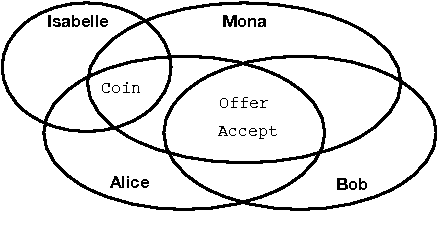
\includegraphics{figure/coin-transfer-visibility.pdf}
\end{center}
\vspace{-2ex}
\caption{Fact Visibility in Coin Transfer Example}
\label{f:CoinTransferVisibility}
\end{figure}

In many practical commercial workflows, it is either not desirable or not legal for all parties to be able to see all data in the system. In the coin transfer example from \S\ref{s:FactsWeights}, it is reasonable to expect that Alice would not want to reveal the total amount of coins she holds to Bob, nor the item she wishes to purchase (the Guitar) to Isabelle. Recall from \S\ref{s:Observation} that a party can see a fact when it is listed in either its \emph{by-authority} set or its \emph{obs-authority} set. We can express this as a simple predicate, where the functions \trm{auth-by} and \trm{auth-obs} retrieve the respective metadata from a fact value.
$$
\trm{sees}~ P~ F = |(\trm{auth-by}~F \cup \trm{auth-obs}~F) \cap \{P\}| \ge 0
$$
Applying this predicate to the initial facts from \S\ref{s:NowWithMetadata} we see that we already have the desired situation. The coin fact and its weight is visible to Alice (the giver), and Mona (the monitor), while the Offer and Accept facts only visible to Alice, Bob and Mona. Figure~\ref{f:CoinTransferVisibility} shows this in diagrammatic form.


% -----------------------------------------------------------------------------
\subsection{Transactions and Validation}
\label{s:Transactions}
Maintaining fact privacy has implications for the underlying implementation. Assume that Alice, Bob, Mona and Isabelle all have their own computers in their own offices that each initially contain the subset of facts that each can see as per Figure~\ref{f:CoinTransferVisibility}. Assume that each party also has a copy of the transfer rule shown in Figure~\ref{f:CoinTransfer}. Now, suppose Alice decides that it is time to perform the transfer. On her own computer she executes the rule while recording the facts that have been consumed and the new facts that have been produced. She then builds a transaction data structure that records this information along with the cryptographic hash of the rule code, which we describe as so:

\begin{small}
\begin{code}
Transaction
{ seq  = ... sequence number ...
, rule = ... hash of code for transfer rule ...
, spent
   = [ Offer  [id    = '1234,
               terms = "To purchase one Guitar"
               giver = !Alice, receiver = !Bob]
        by  {!Bob}              obs {!Mona, !Alice}
        use {'transfer}         num 1

     , Accept [id = '1234, accepter = !Bob]
        by  {!Alice}            obs {!Mona, !Bob}
        use {'transfer}         num 1

     , Coin   [issuer = !Isabelle, holder = !Alice]
        by  {!Isabelle, !Alice} obs {!Mona}
        use {'transfer}         num 1 ]
, new
   = [ Coin   [issuer = !Isabelle, holder = !Bob]
        by  {!Isabelle, !Bob}   obs {!Mona}
        use {'transfer}         num 1 ]
\end{code}
\end{small}

This is the complete transaction that describes all inputs and outputs. Alice can send the complete transaction to Mona, which from Figure~\ref{f:CoinTransfer} is also entitled to see all the input and output facts. In contrast, Isabelle is not entitled to see the Offer fact as she is not listed as either an authorizer or an observer on it. Instead, Alice can compute a \emph{restricted view} of the transaction to send to Isabelle, which enables her to validate that Alice and Bob have authorized the coin facts to be moved, but does not reveal the Offer fact that contains the terms of the transfer.

Curiously, Bob himself is not listed in the metadata of the consumed coin fact, but will be able to infer its contents anyway because according to the transfer rule, the fields must match data in facts that he can see. Alice herself is not listed in the meta-data of the produced coin fact, but will certainly know what this fact is because she is the one forming the transaction. We return to these points in \REF.


% -----------------------------------------------------------------------------
\subsection{Transaction Views and Blinded Hashing}

Alice cannot sent the complete transaction from the previous section to Isabelle, as Isabelle is not entitled to see the contents of the Offer fact. However, Alice does wish Isabelle to know that transfer has taken place, and that Bob has agreed to it, because Isabelle is an authorizer of the Coin facts being moved. To achieve this Alice computes a \emph{restricted view} of the transaction for Isabelle, which consists of a blinded hash of the entire transaction, along with along with a version of the transaction structure where the facts that Isabelle is not entitled to see are replaced by blinded hashes of those facts. A \emph{blinded} hash is a regular cryptographic hash which has been combined with a salt value so that the source data cannot feasibly be recovered by brute force.

For the sake of presentation, lets abbreviate the factoids in the transaction from the previous section as just $d_1, d_2, d_3, d_4$, and write the complete transaction as the following tuple, where we use $h(X)$ to mean the hash of value $X$.
$$
 (seq,~ h(tx), [d_1, d_2, d_3], [d_4])
$$
The above tuple consists of the sequence number, hash of the code for the transaction rule (abbreviated $h(tx)$), a list of factoids being spent, and a list of factoids being created. To compute the blinded hash of the overall transaction we generate a random salt value for each of the factoids, $s_1 .. s_4$, and use it when hashing those factoids.
$$
\begin{array}{rl}
 \hspace{-2ex} h((seq,~ h(tx), [h(d_1, s_1), h(d_2, s_2), h(d_3, s_3)], [h(d_4, s_4)]))
\end{array}
$$
This value is a unique(ish) identifier for the transaction, assuming that the resulting hash values are long enough that we will not see a collision in practice. Now, as Isabelle is entitled to see the Coin facts but not the consumed Offer and Accept facts she receives a view containing the fact data and salt for the Coin facts, but only the blinded hash of the Offer and Accept facts.
$$
\trm{Isabelle:}~~(seq,~ h(tx), [h(d_1, s_1), h(d_2, s_2), (d_3, s_3)], [(d_4, s_4)])
$$
Similarly, Bob is entitled to see the Offer, Accept and produced Coin fact, but not the consumed Coin fact, so receives a corresponding view. Note that Bob can infer what the consumed coin fact will be anyway, but we leave the discussion of this to the next section.
$$
\trm{Bob:}~~(seq,~ h(tx), [(d_1, s_1), (d_2, s_2), h(d_3, s_3)], [(d_4, s_4)])
$$
Finally, Mona is entitled to see everything so she gets the same unblinded transaction that Alice has.
$$
\trm{Mona:}~~(seq,~ h(tx), [(d_1, s_1), (d_2, s_2), (d_3, s_3)], [(d_4, s_4)])
$$
All four parties, including Alice, are then able to use their transaction view to compute the same transaction identifier. Isabelle does not have the data for the Offer and Accept facts, but as she knows their hashes she can still form the hash of the overall transaction. Isabelle also cannot feasibly determine what the Offer and Accept facts originally were because the hashes of these facts have been salted by random numbers $s_1, s_2$ that she does not know. Isabelle \emph{can} determine that the $giver$ and $receiver$ fields of the Offer fact must have been @!Alice@ and @!Bob@ respectively as she knows the rule that the transaction was generated from, and the rule code reveals that these fields must match the corresponding fields in the Coin facts that she does see. Isabelle does not see that a Coin is being transferred @"To purchase on Guitar"@. That information is none of her business.


% -----------------------------------------------------------------------------
\subsection{Consensus}
Once Alice has sent the appropriate restricted transaction view to each party those parties can compare it against their own view of the current ledger state and confirm whether they believe it is valid. Isabelle is able to see the complete number of coins that are currently held by Alice, so Bob can ask Isabelle to confirm that her view of the transaction is valid, and hence enough coins were available for the transfer. In a practical workflow Isabelle would likely represent a commercial Bank, and Bob would trust Isabelle to answer truthfully when asked if enough coins are available for a currency transfer, even though he does not want the Bank to know that he is adding to his collection of guitars. Likewise, Isabelle can ask Bob to confirm that his view of the transaction is valid, and that he really did accept the transfer.

For a concrete implementation there are many ways to manage the transaction confirmation process. For a small number of parties, such as to manage commercial workflows between banks, it could be sufficient for each party to confirm the transaction directly with all others. This would require $O(n^2)$ confirmations in practice, but in the happy case the only information that needs to be exchanged is that the confirming party agrees with the transaction. Each transaction has a unique(ish) identifier consisting of the transaction hash, so each confirmation message is not a large amount of data. For a greater number of parties, cryptographically signed confirmation messages could be propagated with a peer-to-peer protocol, using a spanning tree structure to avoid exchanging a quadratic number of messages~\TODO{cite p2p broadcast work}. In hostile environment such as on the public internet the confirmations could be propagated via Byzantine consensus protocol~\TODO{cite Byzantine work}. Our programming model is not specific to any of the above consensus mechanisms, and different mechanisms are appropriate for different environment, so we do not seek to specify one here.


% -----------------------------------------------------------------------------
\subsection{Authorization Flow}
Note that in our system there is nothing preventing a party from adding a fact to the system which says ``I have a million dollars'', just with their own authority. As mentioned in \label{s:Authority} we allow parties to add arbitrary facts with their own authority, and delete fact that only authorized with their own authority. In the transaction structure of \S\ref{s:Transactions} this is achieved just by leaving the @rule@ field empty, as well as either the @spent@ or @new@ fields. The key property we need to manage is whether anyone else in the system should rightly believe those facts.

 Recall that in the coin transfer example from \S\ref{s:Facts}, the coin facts always carry the authority of multiple parties, which is justified by the sequence of transactions that result in their production. The coin issuer (@Isabelle@ in the example) creates the initial coin facts, specifies the rules for using them, and signs the facts with their own authority. When the coins are transferred onwards the transactions recording the use of the transfer rule are also signed by the parties that propose them. Assuming most parties in the system are honest, invalid transactions will simply not be confirmed. Dishonest parties are free to corrupt their own databases by adding invalid transactions, but honest parties will not accept transactions that do not agree with their own view of the facts.


 As with the consensus mechanism, our programming model does not specify a particular dispute mechanism, as different mechanisms are appropriate for different environments. In a commercial banking system it would be a rare occurrence for a party to actively propose an invalid transaction, so it may be appropriate to pause the system and investigate the issue manually. In a hostile internet environment it maybe instead be appropriate to blacklist the submitting party and not accept further transactions from them.


% -----------------------------------------------------------------------------
\subsection{Incidental Observers}

\TODO{In above transaction the meta-data reveals that it can be formally seen by Isabelle, Bob and Mona, though of course Alice knows about it as she built the transaction}. Distinguish between observer, formal observer, and incidental observer. As Alice is only an incidental observer she should not retain the fact data, as she will not receive information about transactions that spend this fact. Any transactions she might form based on this information may be invalid without her knowing.


% -----------------------------------------------------------------------------
\subsection{Rule Splitting and Nested Transactions}
\TODO{Cite the XA distributed transaction model}. \TODO{Cite Corda Tearoffs}.


% -----------------------------------------------------------------------------
\subsection{Rule Upgrade}
For upgrade, the data model itself does not depend on hashing. In DAML contract ids are hashes that include the code of the template. In Rainfall hashing is used as part of the transaction structure but the fact that fact identity includes the hash of the rule that uses it does not leak into the programming model.






